\renewcommand{\baselinestretch}{2} \small\normalsize
\chapter{Introduction}
This chapter provides the overall objective and introduces the concept of a multistatic RF sensor network in a maritime environment.

\section{Objective}
Analysis of RADAR systems in maritime environments is complicated by the fact that the ocean does not generally provide a smooth or uniform surface to work with. Altitude variations change the aspect angle for multipath bounces, cause wave blockage, and add clutter and spikes to the echo return \cite{skolnik_handbook}, \cite{blake_radar}, \cite{nathanson_radar}. These are random, not deterministic effects which in turn induce signal fluctuations that have a significant impact on the probability of detecting a target. Understanding the impact of the sea surface on propagation is critical to evaluating the performance of a RADAR system in a maritime environment.

When we look at cases where the transmitter and receiver are not colocated, we have a bistatic configuration and analyzing performance becomes even more difficult \cite{willis_bistatic}. Paths are no longer constant, and the clutter and multipath effects get skewed. With multiple receivers or transmitters, the configuration is termed multistatic as there are multiple bistatic elements. Of particular concern here is the case with a single transmitter and multiple receivers.

The objective of this work is to evaluate the performance of multistatic RF sensor networks and demonstrate that Random Matrix Theory (RMT) allows prediction of the signal statistics. The initial step is to generate the multistatic statistics through a Monte Carlo simulation by generating random realizations of ocean surfaces and numerically propagating the RADAR signal. After this, a statistical model based on RMT will be developed.

\section{Multistatic RF Sensor Network Concept}
An example multistatic RF sensor network in a maritime environment is shown in Figure \ref{ms_fig:1}. In this concept, a single transmitter illuminates a target and the echo signal is captured by a pair of receivers. The received signal will fluctuate due to multipath reflections from the surface, path variations, and relative motion of the target. In order to determine the probability of the target being detected by either receiver, we need to understand the statistics of the received signals.

\begin{figure}[H]
  \begin{center}
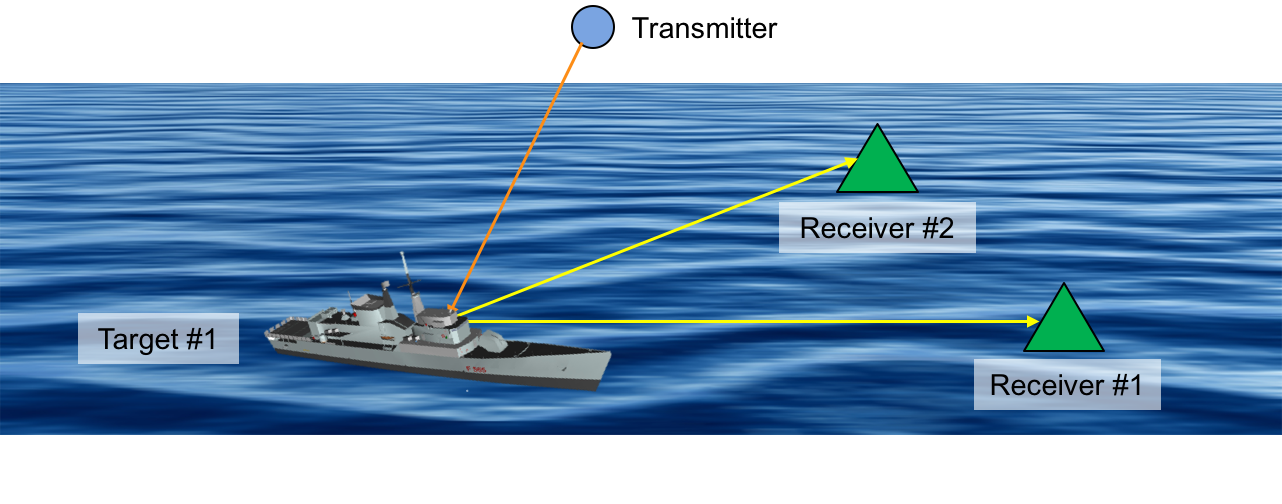
\includegraphics[width=5in]{../media/multistatic/ms_rf_concept.png}
  \end{center}
  \renewcommand{\baselinestretch}{1} \small\normalsize
  \begin{quote}
    \caption[Multistatic RF Sensor Networks Concept]{Multistatic RF Sensor Networks Concept\label{ms_fig:1}}
  \end{quote}
\end{figure}
\renewcommand{\baselinestretch}{2} \small\normalsize
Each receiver observes the target from a different aspect angle than it was illuminated with, resulting in different radiation patterns. The different paths between each receiver also means the impacts from multipath and clutter will be different.